\textbf{6.1.1.} 一电子以 $v = 3.0 \times 10^{7} \mathrm{~m/s}$ 的速率射入磁感强度为 $B$ 的均匀磁场内，速度 $\pmb{v}$ 与 $B$ 垂直， $B$ 的大小为 $B = 10 \mathrm{T}$ . 已知电子的电荷量为 $e = -1.6 \times 10^{-19} \mathrm{C}$ ，质量为 $m = 9.1 \times 10^{-31} \mathrm{~kg}$ . 试求这电子所受的洛伦兹力，并与它在地面所受的重力比较.

\vfill

\textbf{6.1.2.} 一长直导线载有 50A 电流, 在离它 5.0cm 处, 有一电子以速度 v 运动, v 的大小为 $v = 1.0 \times 10^{7}$ m/s, 电子的电荷量为 $e = -1.6 \times 10^{-19}$ C. 试求下列情

况下作用在电子上的洛伦兹力:(1)v平行于导线;(2)v垂直于导线并向着导线;(3)v垂直于导线和电子所构成的平面.

\vfill

\newpage

\textbf{6.1.3.} 试证明:带电粒子在磁场中运动时,磁场作用在它上面的洛伦兹力不

作功.

\vfill

\textbf{6.1.4.} 一电子在 $B = 70\mathrm{Gs}$ 的均匀磁场中作圆周运动，圆的半径为 $r = 3.0\mathrm{cm}$ . 已知电子的质量为 $m = 9.1 \times 10^{-31}\mathrm{kg}$ ，电荷量为 $e = -1.6 \times 10^{-19}\mathrm{C}$ ， $\pmb{B}$ 垂直于纸面向外，电子的轨道在纸面内[图6.1.4(1)]. 设电子某时刻在 $A$ 点，它的速度 $\pmb{v}$ 向上.(1)试画出电子运动的轨道；(2)试求电子的速率 $\pmb{v}$ 和动能 $E_{\mathrm{k}}$ .

图6.1.4(1)
\begin{center}
    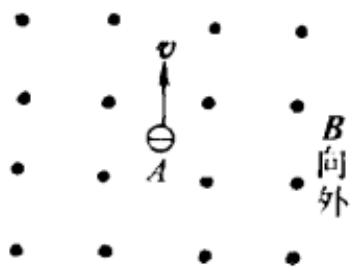
\includegraphics[width=0.5\linewidth]{figures/fig_6_1_4_1.jpg}
\end{center}
\begin{center}
    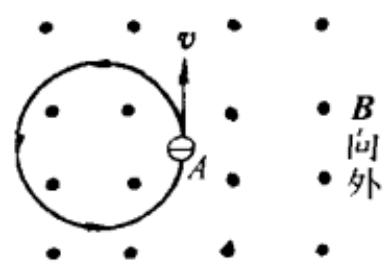
\includegraphics[width=0.5\linewidth]{figures/fig_6_1_4_2.jpg}
\end{center}

\vfill

\newpage

\textbf{6.1.5.} 带电粒子穿过饱和蒸汽时,在它走过的路径上,过饱和蒸汽便凝结成小液滴,从而使得它的运动轨迹(径迹)显示出来,这就是云室的原理.今在一云室中有 B=1.0T 的均匀磁场,观测到一个带电粒子的径迹是一段圆弧,半径为 r=2.0cm;已知这粒子的电荷量为 $1.6 \times 10^{-19}C$ ,质量为 $1.67 \times 10^{-27}kg$ .试求它

的动能.

\vfill

\textbf{6.1.6.} 在极高温度下, 轻原子核由于高速热运动而克服库仑力, 彼此发生结合, 同时放出大量能量, 这种现象称为热核反应. 热核反应的磁约束是用磁场把热核拴住, 使它们不致迅速飞散. 据估算, 氘核需要 $T = 1.2 \times 10^{7} \mathrm{~K}$ 的温度才能发生聚变. 这时要把氘核拴在磁力线上, 回旋半径为 $10 \mathrm{~mm}$ , 试估算所需的磁感强度 $\pmb{B}$ 的值. 已知氘核的质量为 $m = 3.3 \times 10^{-27} \mathrm{~kg}$ , 电荷量为 $e = 1.6 \times 10^{-19} \mathrm{C}$ .

\vfill

\newpage

\textbf{6.1.7.} 测得一太阳黑子的磁场为 B = 4000Gs，试问电子在其中以 $5.0 \times 10^{8}$ cm/s 的速度垂直于 B 运动时，受到的洛伦兹力有多大？回旋半径有多大？已知电子电荷量的大小为 $1.6 \times 10^{-19}$ C，质量为 $9.1 \times 10^{-31}$ kg。

\vfill

\textbf{6.1.8.} 星际空间里某处有 $B = 1.0 \times 10^{-5}\mathrm{Gs}$ 的均匀磁场，一电子在其中作螺旋运动，速度沿 $\pmb{B}$ 的分量为光速 $c$ 的百分之一。试问它沿磁场方向前进一光年（一光年即光走一年的距离）时，它绕磁力线转了多少圈？已知电子的质量为 $9.1 \times 10^{-31}\mathrm{kg}$ ，电荷量的大小为 $1.6 \times 10^{-19}\mathrm{C}$ 。

\vfill

\newpage

\textbf{6.1.9.} 一电子的动能为 $10\mathrm{eV}$ , 在垂直于均匀磁场的平面内作圆周运动. 已知磁场的磁感强度 $B = 1.0\mathrm{Gs}$ , 电子的电荷量 $e = -1.6 \times 10^{-19}\mathrm{C}$ , 质量 $m = 9.1 \times 10^{-31}\mathrm{kg}$ . (1)试求电子的轨道半径 $r$ 和回旋周期 $T$ ; (2)顺着 $\pmb{B}$ 的方向看, 电子是顺时针回旋吗?

\vfill

\textbf{6.1.10.} 一电子在均匀磁场中作圆周运动,频率为 f = 12.0MHz,半径为

53.5cm. 已知电子质量为 $m = 9.11 \times 10^{-31} ~kg$ ，电荷量为 $e = -1.60 \times 10^{-19} ~C$ 。试求：(1) 磁场的磁感强度 B 的值；(2) 电子的动能。

\vfill

\newpage

\textbf{6.1.11.} 一电子的初速度为零, 经过电压 U 加速后, 进入磁感强度为 B 的均匀磁场, 进入磁场时速度为 v, v 与 B 垂直, 如图 6.1.11(1) 所示. 已知电子质量为 m, 电荷量为 e. (1) 试画出电子的轨道; (2) 试求轨道的半径 r; (3) 当 $m = 9.11 \times 10^{-31} ~kg$ , $e = -1.60 \times 10^{-19} ~C$ , U = 3000 V, B = 100 Gs 时, 算出 r 的值.

图6.1.11(1)

\vfill

\textbf{6.1.12.} 已知质子的静质量为 $m_{0}=1.67\times10^{-27}$ kg，电荷量为 $e=1.60\times10^{-19}$ C，地球半径为 6370 km，地球赤道上地面的磁场为 B=0.32 Gs。（1）要使质子在地球磁场的作用下，沿赤道地面作圆周运动，试求质子的速率 v（提示：应考虑狭义相对论效应）；(2) 若要使质子以速率 $v=1.0\times10^{7}$ m/s，沿赤道地面作圆周运动，试问地磁场的磁感强度应该有多大？

\vfill

\newpage

\textbf{6.1.13.} 在一个电视显像管里,电子沿水平方向从南到北运动,动能是 $1.2 \times$

$10^{4}\mathrm{eV}$ . 该处地球磁场在竖直方向上的分量向下, 它的大小是 $B_{\perp} = 0.55\mathrm{Gs}$ . 已知电子的质量为 $m = 9.1 \times 10^{-31}\mathrm{kg}$ , 电荷量为 $e = -1.6 \times 10^{-19}\mathrm{C}$ . 试问: (1) 电子受地磁的作用往哪个方向偏转? (2) 电子的加速度有多大? (3) 电子在电视管内走 20 厘米, 偏转有多大? (4) 地磁对于看电视有没有影响?

\vfill

\textbf{6.1.14.} 一质量为 $m$ 的粒子带有电荷量 $q$ , 以速度 $\pmb{v}$ 射入磁感强度为 $\pmb{B}$ 的均匀磁场中, $\pmb{v}$ 与 $\pmb{B}$ 垂直; 粒子穿过磁场后继续前进, 如图 6.1.14(1) 所示. 已知磁场在 $\pmb{v}$ 方向 (即图中 $x$ 方向) 上的宽度为 $l$ , 粒子从磁场出来后在 $x$ 方向上前进的距离为 $L - \frac{l}{2}$ , 试求粒子的偏转 $y$ ; 当 $l \ll \frac{mv}{qB}$ 时, 结果如何?

\vfill

\newpage

\textbf{6.1.15.} 一质量为 $m$ 、电荷量为 $q$ 的粒子，在 $t = 0$ 时刻，以速度 $\pmb{v} = v_{x}\pmb{i} + v_{z}\pmb{k}$ 自原点 $O$ 出发，在均匀磁场里运动，磁场的磁感强度为 $\pmb{B} = B\pmb{k}$ ，如图6.1.15所示。（1）试求这粒子的运动轨迹；（2）在 $z = a$ 处，有一平面屏，试求这粒子达到屏上的位置。

\vfill

\textbf{6.1.16.} 一质量为 $m$ 、电荷量为 $q$ 的粒子，在磁感强度为 $\pmb{B}$ 的均匀磁场中运动，开始 $(t = 0)$ 时，它的位置和速度分别为 $\pmb{r}_0$ 和 $\pmb{v}_0$ 。试证明：它在 $t$ 时刻的位置为

$$
\begin{array}{r l} \boldsymbol {r} (t) & = \boldsymbol {r} _ {0} + (\boldsymbol {v} _ {0} \cdot \boldsymbol {e} _ {B}) \boldsymbol {e} _ {B} t + \frac {\sin \omega t}{\omega} [ \boldsymbol {e} _ {B} \times (\boldsymbol {v} _ {0} \times \boldsymbol {e} _ {B}) ] \\ & + \frac {1 - \cos \omega t}{\omega} \boldsymbol {v} _ {0} \times \boldsymbol {e} _ {B} \end{array}
$$

式中 $e_{B}$ 是 B 方向上的单位矢量, $\omega = qB/m$ . 它的轨迹是什么曲线?

\vfill

\newpage

\textbf{6.1.17.} 电荷量为 q 的点电荷在磁感强度为 B 的均匀磁场中固定不动；一电子质量为 m、电荷量为 e，在 q 的库仑力作用下，绕 q 作匀速圆周运动，轨道平面与 B 垂直。已知 q 作用在电子上的力的大小等于 B 作用在电子上的力的大小的 N 倍。(1)试求电子的角速度 $\omega$ ; (2)已知 $m = 9.11 \times 10^{-31} ~kg, e = -1.60 \times 10^{-19} ~C$ ，当 $B = 4.27 \times 10^{3} ~Gs, N = 100$ 时，求 $\omega$ 的值。

\vfill

\textbf{6.1.18.} 已知 $\alpha$ 粒子的质量为 $m = 6.7 \times 10^{-27} \mathrm{~kg}$ , 电荷量为 $e = 3.2 \times 10^{-19}$ C. 它在 $B = 1.2 \mathrm{T}$ 的均匀磁场中沿半径为 $45 \mathrm{~cm}$ 的圆周运动. (1) 试求它的速率 $v$ 、动能 $E_{\mathrm{k}}$ 和回旋周期 $T$ ; (2) 若它原来是静止的, 试问要经过多高的电压加速, 它才能达到这个速率?

\vfill

\newpage

\textbf{6.1.19.} 已知氘核的质量比质子大一倍,电荷量与质子相同; $\alpha$ 粒子的质量是质子质量的四倍,电荷量是质子的两倍.(1)试问静止的质子、氘核和 $\alpha$ 粒子经过相同的电压加速后,它们的动能之比是多少?(2)当它们经过这样加速后进入同一均匀磁场,它们都作圆周运动,测得质子圆轨道的半径为 $10\mathrm{cm}$ . 试问氘核和 $\alpha$ 粒子轨道的半径各是多少?

\vfill

\textbf{6.1.20.} 在垂直于均匀磁场的平面内, $\alpha$ 粒子和氘核以相同的初动能沿相同的方向先后从同一点 $P$ 出发, 它们走过半圆形轨道如图 6.1.20 所示, 所用的时间分别是 $t_{c}$ 和 $t_{d}$ . 已知 $\alpha$ 粒子的质量比氘核大一倍, 电荷量也比氘核大一倍. 试判断图中到达 $S$ 点的是哪一个? 并求比值 $t_{a} / t_{d}$ .
\begin{center}
    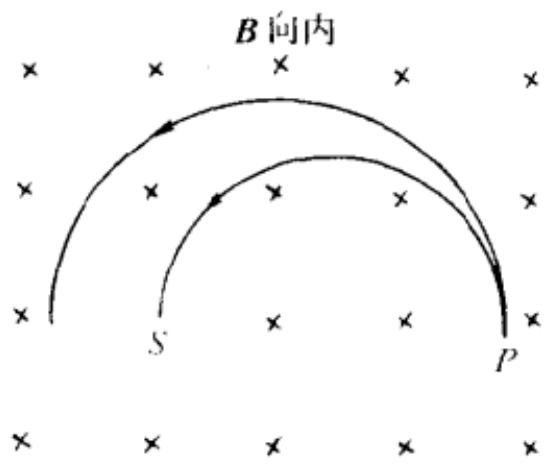
\includegraphics[width=0.5\linewidth]{figures/fig_6_1_20.jpg}
\end{center}

\vfill

\newpage

\textbf{6.1.21.} 一氘核在 $B = 1.5\mathrm{T}$ 的均匀磁场中运动，轨迹是半径为 $40\mathrm{cm}$ 的圆周。已知氘核的质量为 $3.34\times 10^{-27}\mathrm{kg}$ ，电荷量为 $1.60\times 10^{-19}\mathrm{C}$ 。（1）试求氘核的速度和走半圈所需的时间；(2)需要多高的电压才能把氘核从静止加速到这个速度？

\vfill

\textbf{6.1.22.} 一质谱仪的构造原理如图6.1.22所示，离子源 $S$ 产生质量为 $m$ 、电荷量为 $q$ 的离子，离子产生出来时速度很小，可以看作是静止的；离子产生出来后经过电压 $U$ 加速，进入磁感强度为 $B$ 的均匀磁场，沿着半圆周运动而到达记录它的底片 $P$ 上，测得它在 $P$ 上的位置到入口处的距离为 $x$ . (1)试证明这粒子的质量为 $m = \frac{qB^2}{8U} x^2$ ; (2)用钠离子做实验，得到如下数据： $U = 705\mathrm{V}, B = 3580\mathrm{Gs}, x = 10\mathrm{cm}$ . 试求钠离子的荷质比 $q / m$ .

\vfill

\newpage

\textbf{6.1.23.} 已知碘离子所带电荷量为 $q=1.6\times10^{-19}C$ ，它在 $B=4.5\times10^{-2}T$ 的均匀磁场中作圆周运动时，回旋七周的时间为 $1.29\times10^{-3}s$ 。试求碘离子的质量。

\vfill

\textbf{6.1.24.} 在粒子的速度比光速 c 小得多的情况下, 粒子的质量可当作与速度无关. 试证明: 这时 D 形回旋加速器交变电压的频率与带电粒子作圆周运动的半径无关.

\vfill

\newpage

\textbf{6.1.25.} 回旋加速器的构造原理如图 6.1.25 所示, 用它加速电荷量为 q、质量为 m 的粒子, 其加速电压 U 和磁感强度 B 均为已知. 设粒子开始时动能很小, 可略去不计. 试问将粒子加速到动能为 $E_{k}$ , 需要多长时间?

\vfill

\textbf{6.1.26.} 一回旋加速器 $D$ 形电极圆周的最大半径为 $60\mathrm{cm}$ ，用它来加速质量为 $1.67 \times 10^{-27}\mathrm{kg}$ 、电荷量为 $1.6 \times 10^{-19}\mathrm{C}$ 的质子，要把质子从静止加速到 $4.0\mathrm{MeV}$ 的能量。(1)试求所需的磁感强度 $\pmb{B}$ 的值；(2)设两 D 形电极间的距离为 $1.0\mathrm{cm}$ ，加速电压为 $2.0 \times 10^{4}\mathrm{V}$ ，其间电场是均匀的，试求加速到上述能量所需的时间。

\vfill

\newpage

\textbf{6.1.27.} 一电子在 $B = 20\mathrm{Gs}$ 的磁场里沿半径为 $R = 20\mathrm{cm}$ 的螺旋线运动, 螺距为 $h = 5.0\mathrm{cm}$ , 如图6.1.27所示. 已知电子的荷质比为 $\left|e\right| / m = 1.76 \times 10^{11}\mathrm{C/kg}$ , 试求这电子的速度.

\vfill

\textbf{6.1.28.} 动能为 2000eV 的正电子在 B=1000Gs 的均匀磁场中运动, 它的速度 v 与 B 成 $89^{\circ}$ 角, 所以它的轨迹是一条螺旋线, 如图 6.1.28 所示. 已知正电子的质量为 $m=9.11\times10^{-31}kg$ , 电荷量为 $e=1.60\times10^{-19}C$ . 试求这螺旋运动的周期 T、半径 r 和螺距 p.

\vfill

\newpage

\textbf{6.1.29.} 粒子速度选择器(或称滤速器)是由互相正交的均匀电场 E 和均匀磁场 B 构成的, 各种速度的粒子射入时, 速度都与 E 正交, 也都与 B 正交, 如图 6.1.29 所示.(1)试说明: 当入口和出口都很小时, 只有速度的大小 $v_{c}$ 为某一值的粒子才能通过, 而其他的便都不能通过.(2)当 $E = 3.0 V/m, B = 10 G s$ 时, 试计算通过的粒子的速率 $v_{c}$ . (3)带电粒子的电荷量 q 的大小有没有影响? (4)带电粒子的电荷是正还是负有没有影响?

图6.1.29
\begin{center}
    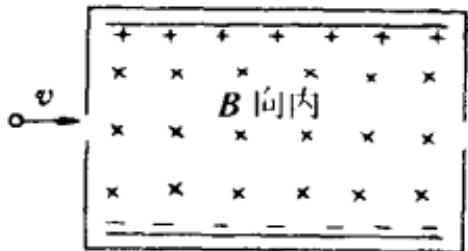
\includegraphics[width=0.5\linewidth]{figures/fig_6_1_29.jpg}
\end{center}

\vfill

\textbf{6.1.30.} 空间某一区域里有 $E = 1500\mathrm{V / m}$ 的电场和 $B = 4000\mathrm{Gs}$ 的磁场，这两个场作用在一个运动电子上的合力为零。当电子的速度 $\pmb{v}_{\perp}\pmb{B}$ 时，试求这个电子的速率 v，并画出 E、B 和 v 三者的相互方向.

图6.1.30
\begin{center}
    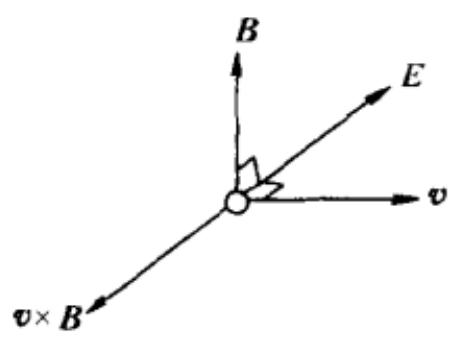
\includegraphics[width=0.5\linewidth]{figures/fig_6_1_30.jpg}
\end{center}

\vfill

\newpage

\textbf{6.1.31.} 空间某一区域有均匀磁场,磁感强度 B 沿 x 轴方向.一带电粒子(质量为 m、电荷量为 q)在这磁场中运动,开始时,速度为 $v_{0}$ , $v_{0}$ 与 z 轴垂直, $v_{0}$ 与 B 之间的夹角为 $\alpha$ ;位置为 $x_{0}=y_{0}=0$ , $z_{0}=mv_{0}\sin\alpha/qB$ .试求这粒子的运动轨迹.

\vfill

\textbf{6.1.32.} 空间某一区域有均匀电场 E 和均匀磁场 B, E 和 B 的方向相同, 一电子(质量为 m、电荷量为 e)在这场中运动, 试分别求下列情况下电子的加速度和电子的轨迹: 开始时(1) $v_{0}$ 与 E 方向相同; (2) $v_{0}$ 与 E 方向相反; (3) $v_{0}$ 与 E 垂直.

\vfill

\newpage

\textbf{6.1.33.} 一无限大平行板电容器充电后,两极板间产生一均匀电场 E, 另有一均匀磁场 B 与 E 垂直, 如图 6.1.33(1) 所示. 一电子(质量为 m, 电荷量为 e) 从负极板出来, 初速度很小, 可当作零. 不考虑重力. 试证明: 当两极板间的距离 $d > \frac{2mE}{|e|B^{2}}$ 时, 它不可能到达正极板.

图6.1.32(4)
\begin{center}
    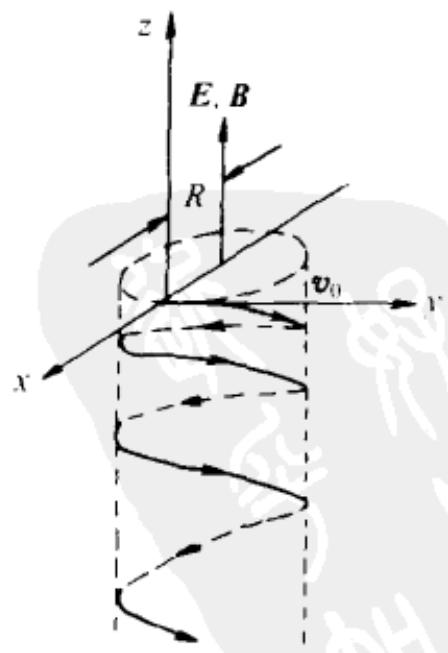
\includegraphics[width=0.5\linewidth]{figures/fig_6_1_33.jpg}
\end{center}

\vfill

\textbf{6.1.34.} 在空间有互相垂直的均匀电场 E 和均匀磁场 B, B 沿 x 轴方向, E 沿 z 轴方向. 一电子 (质量为 m, 电荷量为 e) 开始从原点出发, 以速度 $v_{0}$ 向 y 轴方向前进, 如图 6.1.34 所示. 试求这电子运动的轨迹.

\vfill

\newpage

\textbf{6.1.35.} 设氢原子中的电子沿半径为 $r$ 的圆轨道绕原子核运动, 若把氢原子放在磁感强度为 $\pmb{B}$ 的磁场中, 使电子的轨道平面与 $\pmb{B}$ 垂直, 假定 $r$ 不因 $\pmb{B}$ 而改变, 则当观测者顺着 $\pmb{B}$ 的方向看时, (1) 若电子是沿顺时针方向旋转, 试问电子的角频率(角速度)是增大还是减小? (2) 若电子是沿逆时针方向旋转, 试问电子的角频率是增大还是减小?

\vfill

\textbf{6.1.36.} 设电子质量为 $m$ ，电荷量为 $e$ ，以角速度 $\omega$ 绕带正电的质子作圆周运动。当加上外磁场 $\pmb{B}, \pmb{B}$ 的方向与电子轨道平面垂直时，设电子轨道半径不变，而角速度则变为 $\omega'$ 。试证明：电子角速度的变化近似等于

$$
\Delta \omega = \omega^ {\prime} - \omega = \pm \frac {1}{2} \frac {e}{m} B
$$

\vfill

\newpage

\textbf{6.1.37.} 一铜片厚为 $d = 1.0\mathrm{mm}$ , 放在 $B = 1.5\mathrm{T}$ 的磁场中, 磁场方向与铜片表面垂直, 如图6.1.37所示. 已知铜片里每立方厘米有 $8.4 \times 10^{22}$ 个自由电子, 每个电子的电荷量为 $e = -1.6 \times 10^{-19}\mathrm{C}$ . 当铜片中有 $I = 200\mathrm{A}$ 电流时, 试求铜片两侧的电势差 $U_{ab}$ .

\vfill

\textbf{6.1.38.} 一块样品如图 6.1.38, 已知它的横截面积为 S, 宽为 l, 载有电流 I. 外磁场的磁感强度为 B, B 与电流 I 垂直. 设样品单位体积内有 n 个载流子, 每个载流子的电荷量为 q, 平均定向速率为 u. (1) 试证明, 这块样品中存在一个大小为

E = uB 的电场; 并指出 E 的方向; (2) 试求样品两侧的电势差 $U_{ab}$ ; 哪侧电势高? (3) 霍尔系数定义为 $R = \frac{ES}{IB}$ , 试证明: $R = \frac{1}{nq}$ ; (4) 试证明: $R = \frac{u_{m}}{\sigma}$ , 式中 $u_{m}$ 是载流子的迁移率(即单位电场强度所产生的平均定向速率), $\sigma$ 是样品的电导率.
\begin{center}
    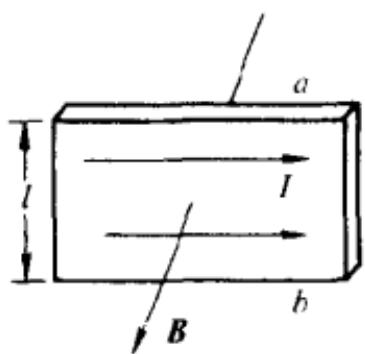
\includegraphics[width=0.5\linewidth]{figures/fig_6_1_38.jpg}
\end{center}

\vfill

\newpage

\textbf{6.1.39.} 一块半导体样品的体积为 $a \times b \times c$ ，如图6.1.39所示，载有电流 $I$ ，处在磁场强度为 $H$ 的外磁场中， $I$ 沿 $x$ 轴方向， $H$ 沿 $z$ 轴方向。由实验测得的数据为 $a = 0.10\mathrm{cm}$ ， $I = 1.0\mathrm{mA}$ ， $H = 300\mathrm{Oe}$ ，片两侧的电势差为 $U_{AB} = 6.55\mathrm{mV}$ 。（1）试问这半导体是正电荷导电(p型)还是负电荷导电(n型)?(2)设每个载流子电荷量的大小为 $q = 1.60 \times 10^{-19}C$ ，试求载流子浓度（即单位体积内参加导电的带电粒子数）.

图6.1.39
\begin{center}
    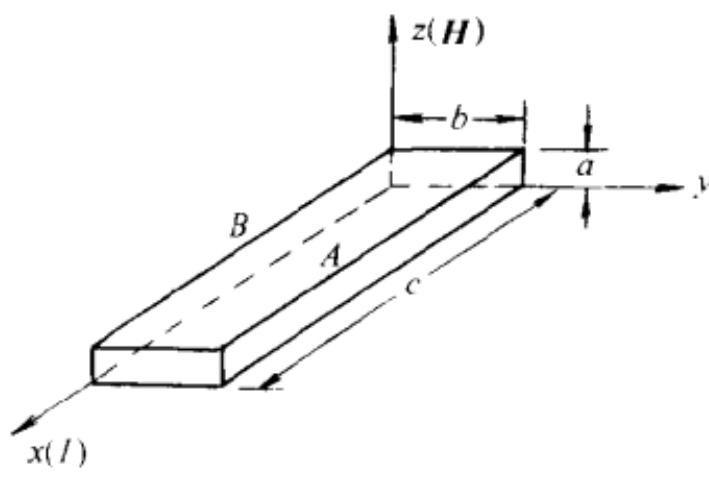
\includegraphics[width=0.5\linewidth]{figures/fig_6_1_39.jpg}
\end{center}

\vfill

\textbf{6.1.40.} 一铜导线载有电流 I, I 均匀分布在它的横截面上; 已知导线横截面的半径为 R, 铜内参加导电的自由电子数密度为 n, 电子的电荷量为 e. 试求这导线的轴线与表面的电势差 U. 当 $R = 5.0 \, mm, I = 50 \, A, n = 8.4 \times 10^{22} \, \text{个}/(\text{cm})^3, e = -1.6 \times 10^{-19} \, \text{C}$ 时, 试计算 U 的值.

\vfill

\newpage

\textbf{6.1.41.} 把载流铜片放在 $B = 100 ~m T$ 的外磁场中, 测量它的霍尔效应, 测得纵向电场强度是横向电场强度的 $n = 3.1 \times 10^{3}$ 倍. 试求这铜片中载流子的迁移率 (单位电场强度所产生的平均定向速率).

\vfill

\textbf{6.1.42.} 在宽为 $b$ 、厚为 $d$ 的半导体样品中，有沿长度方向流动的电流 $I$ ；外加一垂直于 $I$ 的横向磁场，磁感强度为 $\pmb{B}$ ，如图6.1.42所示。设样品中单位体积内有n 个载流子参加导电, 每个载流子的电荷量为 $e = 1.6022 \times 10^{-19} C$ . (1) 试求样品两侧的电势差 $U_{H} = U_{A} - U_{A'}$ 和霍尔电阻 $R_{H} = U_{H}/I$ ; (2) 1985 年, 克利青 (K.V.Klitzing) 发现, 霍尔电阻是量子化的, 即

图6.1.42

$$
R _ {H} = \frac {h}{i e ^ {2}}
$$

式中 $i=1,2,3,\cdots;h=6.6261\times10^{-34}J\cdot s$ 是普

朗克常量. 通常把 $R_{k} = \frac{h}{e^{2}}$ 叫做量子化霍尔电阻(或克利青常量), 它是一个基本物理常量. 试由 $h$ 和 $e$ 的单位和数值求 $R_{k}$ 的单位和数值.
\begin{center}
    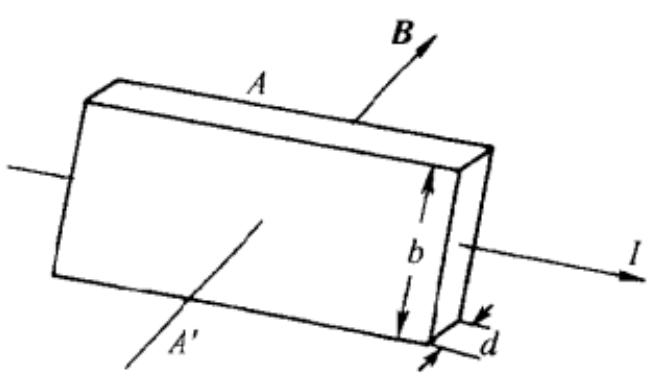
\includegraphics[width=0.5\linewidth]{figures/fig_6_1_42.jpg}
\end{center}

\vfill

\newpage

\textbf{6.2.3.} 有一段长为 $l$ 的直导线, 质量为 $m$ , 用细丝线平挂在磁感强度为 $\pmb{B}$ 的外磁场中, 导线中载有电流 $I, I$ 的方向与 $\pmb{B}$ 垂直, 如图6.2.3所示. (1)试求丝线中张力为零时的电流 $I$ ; 当 $l = 50\mathrm{cm}, m = 10\mathrm{g}, B = 1.0\mathrm{T}$ 时, $I = ?$ (2)在什么条件下导线会向上运动?
\begin{center}
    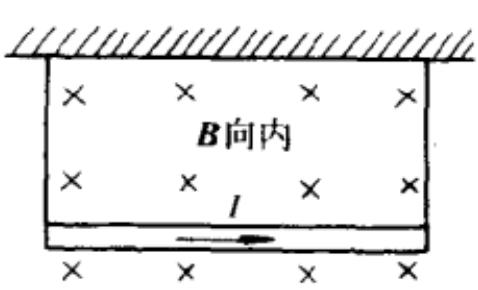
\includegraphics[width=0.5\linewidth]{figures/fig_6_2_3.jpg}
\end{center}

\vfill

\textbf{6.2.4.} 一铜线弯成 $\square$ 形, 如图 6.2.4(1) 所示, 其中 $OA$ 段和 $DO'$ 段固定在水平方向不动, $ABCD$ 段是边长为 $l$ 的正方形的三边, 可以绕 $OO'$ 转动;整个导线放在均匀外磁场中,磁感强度 B 竖直向上.已知铜线的横截面积为 $S=2.0mm^{2}$ , 铜的密度为 $8.9g/cm^{2}$ . 当这铜线中的电流为 I=10A 时, 在平衡情况下, AB 段和 CD 段与竖直方向的夹角为 $\alpha=15^{\circ}$ . 试求磁感强度 B 和磁场强度 H 的大小.
\begin{center}
    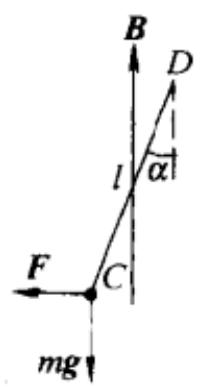
\includegraphics[width=0.5\linewidth]{figures/fig_6_2_4.jpg}
\end{center}

\vfill

\newpage

\textbf{6.2.5.} 一质量为 $m$ 的导线 $AB$ , 水平地架在倾角为 $\theta$ 的两金属片 $C$ 和 $D$ 上, 两片相距为 $l$ , 并维持一定的电势差, 因而导线中有电流 $I_1$ 流过. 在下边有一条固定的无穷长直水平导线, 载有电流 $I_2$ . 两导线构成的平面与金属片的斜面重合, 如图 6.2.5 所示. 设电源离 $AB$ 很远, 联接电源的导线中的电流对 $AB$ 的作用力可略去不计, $AB$ 与 $C, D$ 间的摩擦力亦可略去不计. 试求 $AB$ 静止时, 两导线间的距离 $d$ .

图6.2.5
\begin{center}
    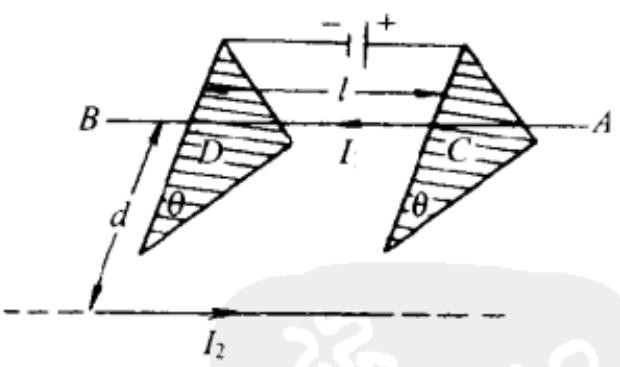
\includegraphics[width=0.5\linewidth]{figures/fig_6_2_5.jpg}
\end{center}

\vfill

\textbf{6.2.6.} 一均匀圆柱体的质量为 $m$ ，半径为 $R$ ，长为 $l$ ，它上面绕有 $N$ 匝外皮绝缘的细导线，导线与圆柱体的轴线共面。这圆柱体放在倾角为 $\theta$ 的斜面上，轴线是水平的，导线中通有电流 $I$ ，整个圆柱体都处在均匀外磁场中，磁感强度 $B$ 的方向竖直向上。当线圈的平面与斜面夹角为 $\varphi$ 时，圆柱体正好静止不动，如图6.2.6(1)所示。设导线的质量可略去不计，试求导线中电流的大小和方向。


图6.2.6(1)
图6.2.6(2)
\begin{center}
    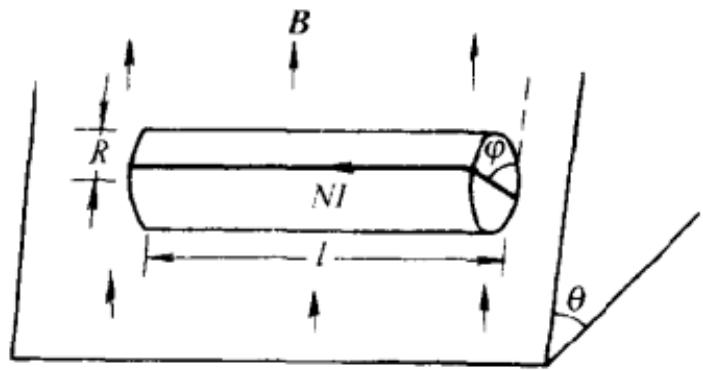
\includegraphics[width=0.5\linewidth]{figures/fig_6_2_6_1.jpg}
\end{center}
\begin{center}
    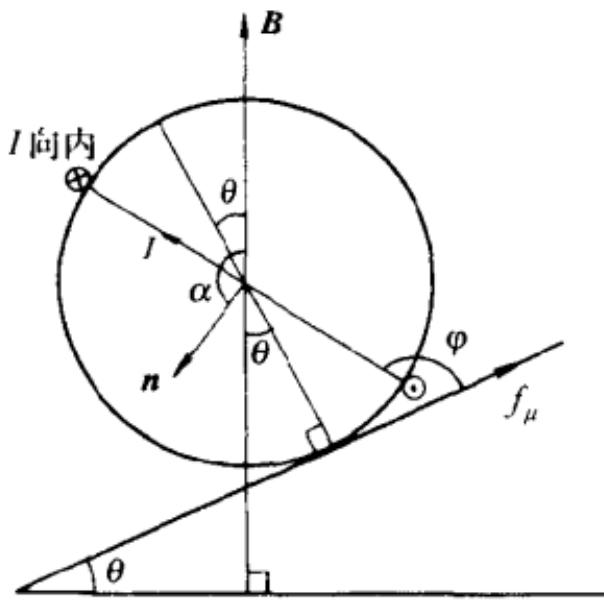
\includegraphics[width=0.5\linewidth]{figures/fig_6_2_6_2.jpg}
\end{center}

\vfill

\newpage

\textbf{6.2.7.} 质量为 $m$ 的一段导线弯成 $\square$ 形, 上面一段长为 $l$ , 处在磁感强度为 $\pmb{B}$ 的均匀外磁场中, $\pmb{B}$ 与导线垂直; 导线下面两端分别插在两水银杯里, 两杯水银则与一带开关 $\mathbf{K}$ 的电源联接, 如图 6.2.7 所示. 当 $\mathbf{K}$ 一接通, 导线便会从水银杯里跳起来. 设跳起的高度为 $h$ , 试求通过导线的电荷量 $q$ , 并计算 $m = 10g, l = 20cm, h = 3.0m, B = 0.10T$ 时 $q$ 的值.

\vfill

\textbf{6.2.8.} 一电流秤如图 6.2.8 所示, 它的一臂下面挂有一个矩形线圈, 共有九匝, 这线圈的下部悬在磁感强度为 B 的均匀外磁场内, 下边长为 l 的一段与 B 垂直. 当线圈的导线中通有电流 I 时, 调节砝码使两臂达到平衡; 然后使电流反向, 但大小仍为 I, 这时需要在一臂上加质量为 m 的砝码, 才能使两臂再达到平衡. 试求磁感强度的大小 B, 并计算当 $l = 10.0 \, cm, I = 0.100 \, A, m = 8.78 \, g$ 时 B 的值.
\begin{center}
    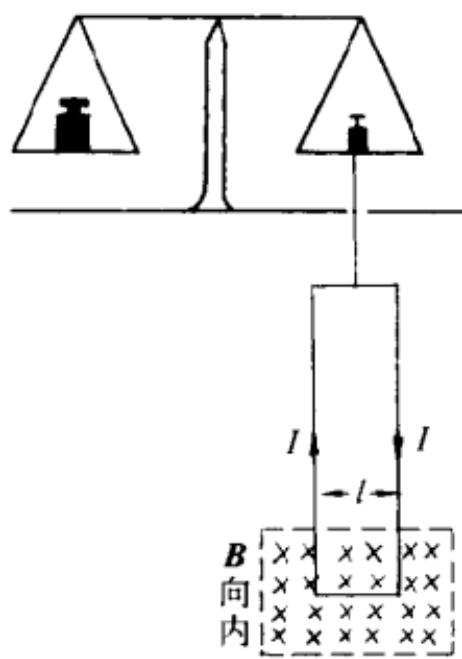
\includegraphics[width=0.5\linewidth]{figures/fig_6_2_8.jpg}
\end{center}

\vfill

\newpage

\textbf{6.2.9.} 空间某处有两个磁场, 它们的磁场强度分别为 $H_{1}$ 和 $H_{2}, H_{1}$ 和 $H_{2}$ 都在水平方向, $H_{1}$ 向北, 大小为 $H_{1}=1.73Oe; H_{2}$ 向东, 大小为 $H_{2}=1.00Oe$ . 现在该处有一段载流直导线, 试问它应如何放置, 才能使两磁场作用在它上面的合力为零?

\vfill

\textbf{6.2.10.} 一段直导线长为 l = 10cm，载有 I = 10 安培的电流，处在磁感强度为

B 的均匀外磁场中，B 与电流垂直，B 的大小为 B = 30Gs. (1) 试求磁场作用在这段导线上的力 F 的大小；(2) 当这段导线以 25cm/s 的速率逆 F 的方向运动时，试求 F 作功的功率 P.

\vfill

\newpage

\textbf{6.2.11.} 一正方形线圈由外皮绝缘的细导线绕成,共绕有200匝,每边长为150mm,放在磁感强度为4.0T的外磁场中.当导线中通有I=8.0A的电流时,试求:(1)作用在线圈上的力矩 $M=m\times B$ 的最大值;(2)线圈的磁矩m的值.

\vfill

\textbf{6.2.12.} 一矩形线圈由表面绝缘的细导线密绕而成,共10匝,矩形边长分别为10.0cm和5.0cm,导线中载有0.10A的电流,这线圈可以绕它的一边 $OO'$ 转动,如图6.2.12(1)所示.当加上磁感强度为B的均匀外磁场,B与线圈平面成30°角,B的大小为0.50T时,试求使这线圈转动的力矩.

\vfill

\newpage

\textbf{6.2.13.} 一矩形线圈长 20mm, 宽 10mm, 由外皮绝缘的细导线密绕而成, 共有 1000 匝, 放在 B = 1000Gs 的均匀外磁场中, 当导线中通有 100mA 的电流时, 试求图 6.2.13 中两种情况下线圈各边所受的安培力之和 F 以及线圈所受的力矩 M: (1) B 与线圈平面的法线平行; (2) B 与线圈平面的法线垂直.

\vfill

\textbf{6.2.14.} 一边长为 $a$ 的正方形线圈载有电流 $I$ , 处在磁感强度为 $\pmb{B}$ 的均匀外磁场中, $\pmb{B}$ 沿水平方向, 线圈可以绕通过中心的竖直轴 $OO'$ (图6.2.14) 转动, 转动惯量为 $J$ . 略去轴承上的摩擦, 试求这线圈围绕平衡位置作微小振动的周期 $T$ .

\vfill

\newpage

\textbf{6.2.15.} 一导线每厘米长的质量为 $0.10\mathrm{g}$ , 作成一个矩形线圈 abcd, 边长分别为 $8.0\mathrm{cm}$ 和 $6.0\mathrm{cm}$ , 如图 6.2.15(1) 所示, 它可以绕 ab 边自由转动, 图中 $z - x$ 平面为水平面, 整个线圈处在磁感强度为 $\pmb{B}$ 的均匀外磁场中, $\pmb{B}$ 沿 $y$ 轴方向. 当线圈中载有 $I = 10\mathrm{A}$ 电流时, 线圈离开垂直位置, 偏转 $30^{\circ}$ 角. (1) 试求磁感强度 $\pmb{B}$ 的值; (2) 如果 $\pmb{B}$ 的方向不是沿 $y$ 轴, 而是沿 $x$ 轴, 线圈将如何?

图6.2.15(1)
\begin{center}
    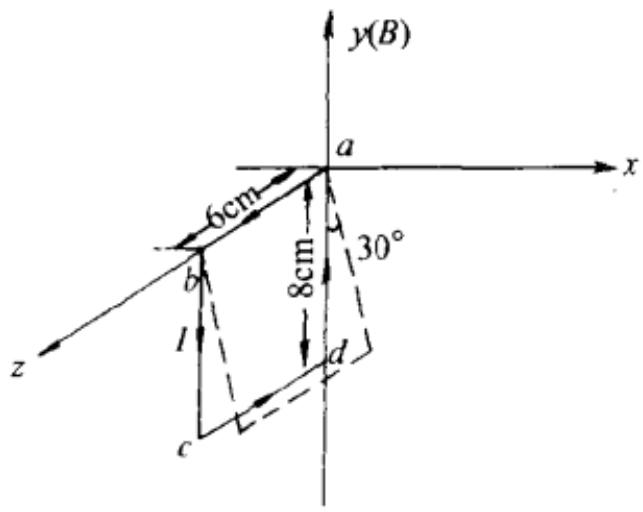
\includegraphics[width=0.5\linewidth]{figures/fig_6_2_15_1.jpg}
\end{center}
\begin{center}
    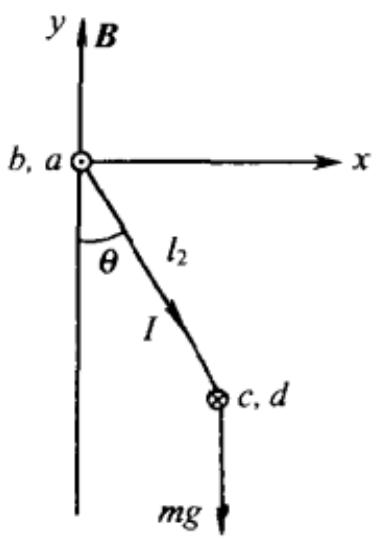
\includegraphics[width=0.5\linewidth]{figures/fig_6_2_15_2.jpg}
\end{center}

\vfill

\textbf{6.2.16.} 永磁式电流计的主要部分是在永磁场中装一个可以转动的矩形线圈, 线圈的转轴上装有螺旋形弹簧; 轴的上端安有一根随轴转动的指针, 当电流通过线圈时, 指针便随着线圈转动到一定位置; 为了使线圈转动的范围内各处的磁场大小都一样, 让线圈套在一个圆柱形的软铁心上, 如图 6.2.16 所示. 设线圈长为 $a$ , 宽为 $b$ , 共有 $N$ 匝, 当它的导线中通有电流 $I$ 时, 指针偏转的角度为 $\theta$ , 永磁场的磁感强度大小为 $B$ . (1) 试求磁场作用在线圈上的力矩 $M$ 和弹簧的扭转系数 $K$ ; (2) 当 $B = 2000\mathrm{Gs}, a = 2.0\mathrm{cm}, b = 1.0\mathrm{cm}, N = 250$ 匝, $I = 0.10\mathrm{mA}$ 时, $\theta = 30^{\circ}$ , 试计算 $K$ 的值.

(1) 主视图

(2) 俯视图
图6.2.16
\begin{center}
    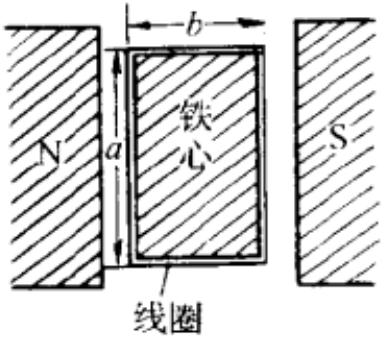
\includegraphics[width=0.5\linewidth]{figures/fig_6_2_16_1.jpg}
\end{center}
\begin{center}
    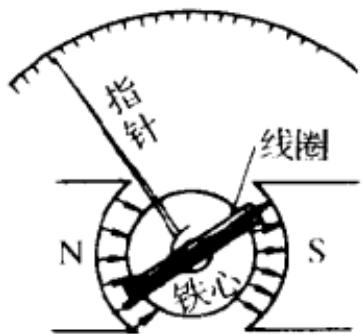
\includegraphics[width=0.5\linewidth]{figures/fig_6_2_16_2.jpg}
\end{center}

\vfill

\newpage

\textbf{6.2.17.} 一永磁式电流计中线圈面积为 $6.0\mathrm{cm}^2$ ，由50匝表面绝缘的细导线密绕而成；线圈平面的法线在水平方向，线圈可以绕固定的竖直轴 $OO^{\prime}$ 转动，永磁体的磁感强度 $\pmb{B}$ 与转轴 $OO^{\prime}$ 垂直并成辐射状，如图6.2.17所示.线圈的 $ab$ 边和cd边所在处的 $B = 100\mathrm{Gs}$ ，导线中通有 $1.0\mathrm{mA}$ 的电流.设线圈轴上游丝的扭转系数为 $K = 0.10\mathrm{dyn}\cdot \mathrm{cm}/$ 度，试求线圈偏转的角度.

\vfill

\textbf{6.2.18.} 台式或墙式电流计是一种很灵敏的电流计,它的矩形线圈由金属丝悬挂在圆柱形铁心和永磁铁之间的狭缝里,这狭缝里的磁力线是辐射状的;金属丝上固定了一个小反

(1) 立体图
(2) 俯视图
图6.2.17

光镜, 镜前有照明光源和圆弧形标尺(圆弧的中心在线圈的转轴上), 如图 6.2.18 所示. 当线圈内有电流 $I$ 通过时, 线圈便受力而转动. 已知线圈是由表面绝缘的细导线密绕而成, 长为 $a = 3.0\mathrm{cm}$ , 宽为 $b = 1.0\mathrm{cm}$ , 共有 100 匝. 金属丝的扭转系数为 $1.0 \times 10^{-5}$ 克力·厘米/度, 磁场强度为 $H = 1000\mathrm{Oe}$ , 弧尺的半径为 $R = 1.00\mathrm{m}$ . (1) 试求电流 $I = 1.0\mu \mathrm{A}$ 时, 磁场作用在线圈上的力矩 $M$ 和线圈的偏转角度 $\theta$ ; (2) 当弧尺上的光点偏转为 $1.0\mathrm{mm}$ 时, 通过电流计的电流是多少?

(1) 立体图

(2) 俯视图
图6.2.18
\begin{center}
    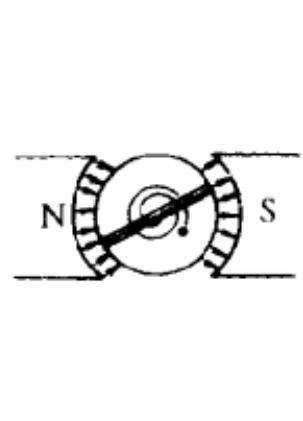
\includegraphics[width=0.5\linewidth]{figures/fig_6_2_18_1.jpg}
\end{center}
\begin{center}
    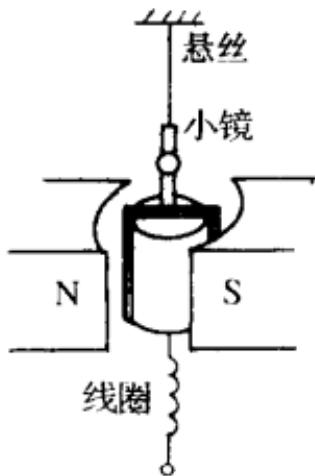
\includegraphics[width=0.5\linewidth]{figures/fig_6_2_18_2.jpg}
\end{center}
\begin{center}
    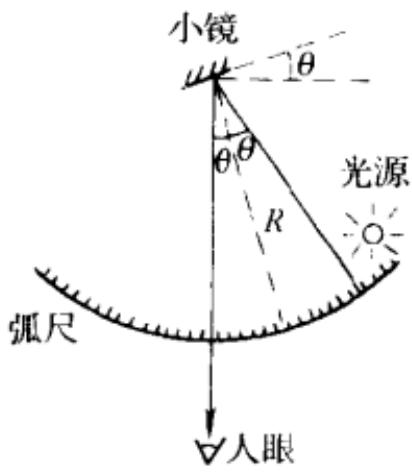
\includegraphics[width=0.5\linewidth]{figures/fig_6_2_18_3.jpg}
\end{center}

\vfill

\newpage

\textbf{6.2.19.} 一万用电表的表头是一只磁电式电表,它的矩形线圈长 $11\mathrm{mm}$ , 宽 $10\mathrm{mm}$ , 由 1500 匝表面绝缘的导线绕成; 线圈游丝的扭转系数为 $2.2 \times 10^{-8}\mathrm{N} \cdot \mathrm{m}/$ 度. 若表头的最大偏转角为 $90^{\circ}$ , 表头的灵敏度 (即最大偏转时的电流) 为 $40\mu \mathrm{A}$ , 试求线圈所在处 (即磁铁的空隙中) 的磁感强度.

\vfill

\textbf{6.2.20.} 一半径为 R=0.10 米的半圆形线圈, 载有电流 I=10 安培, 放在均匀外磁场中, 磁场强度 H 的大小为 $H=5.0 \times 10^{3}Oe$ , 方向与线圈平面平行, 如图 6.2.20(1) 所示。(1) 试求线圈所受力矩的大小和方向; (2) 在这力矩的作用下, 线圈转 $90^{\circ}$ (即转到线圈平面与 H 垂直), 设在转动过程中, 线圈中的电流不变, 试求力矩作的功.

\vfill

\newpage

\textbf{6.2.21.} 一导线做成的圆环, 半径为 R, 载有电流 I, 放在磁感强度为 B 的均匀外磁场中, B 与圆环的轴线平行并沿电流 I 的右旋进方向. 试求 B 在导线内产生的张力.

图6.2.21(1)
\begin{center}
    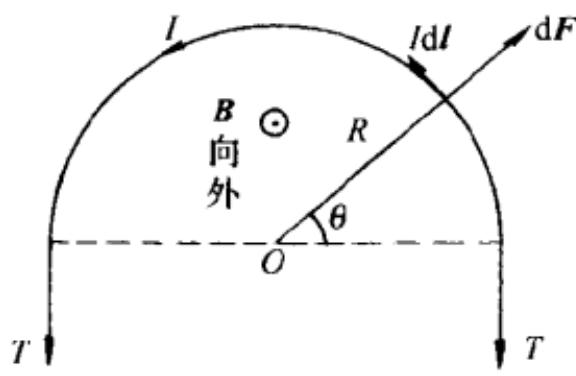
\includegraphics[width=0.5\linewidth]{figures/fig_6_2_21.jpg}
\end{center}

\vfill

\textbf{6.2.23.} 一条很长的绝缘体圆柱,外面包有一层很薄的金属膜,金属膜载有沿轴线方向流动的电流 I,已知电流均匀分布在金属膜里.试求由于电流引起的、金属膜对绝缘柱的压强.

\vfill

\newpage

\textbf{6.2.24.} 一很长的直螺线管由外表绝缘的细导线在塑料管上密绕而成, 单位长度的匝数为 $n$ . 当导线中通有电流 $I$ 时, 略去边缘效应 (即将螺线管当成无限长), 试求导线因电流而对塑料管施加的压强.

\vfill

\textbf{6.2.25.} 半径为 $R = 10\mathrm{cm}$ 的圆线圈由表面绝缘的细导线密绕而成，共绕有2000匝.当导线中通有2.0A的电流时，加上磁感强度为 $\pmb{B}$ 的外磁场， $\pmb{B}$ 的方向与线圈平面平行, B 的大小为 $5.0 \times 10^{-2} ~T$ , 试求磁场作用在线圈上的力矩 M.

\vfill

\newpage

\textbf{6.2.26.} 一螺线管横截面的直径为 $15\mathrm{mm}$ , 由表面绝缘的细导线密绕而成, 共绕有 2500 匝. (1) 当导线中通有 $2.0\mathrm{A}$ 的电流时, 试求这螺线管的磁矩; (2) 将这载流螺线管放到 $B = 4.0\mathrm{T}$ 的均匀外磁场中, 试求它所受力矩的最大值.

\vfill

\textbf{6.2.27.} 试证明: 在均匀外磁场中, 任何一个闭合电流环路所受到的安培力的主矢(即电流环路各部分所受的安培力之和)为零.

\vfill

\newpage

\textbf{6.2.28.} 1820年9月,安培听到奥斯特发现电流可以使磁针偏转的消息后,便想到电流之间也可能有相互作用力.在一个星期里,他就用实验证明了他的想法是对的.可是当时有人说:既然两个电流都与磁针有相互作用力,则两个电流之间必定有相互作用力;因此,安培的实验是多余的.你认为这人的说法怎么样?

\vfill

\textbf{6.2.29.} 一无穷长直导线载有电流 $I$ , 离这导线为 $r$ 处有一小磁针, 这小磁针可以绕它的固定中心自由转动. 试证明: 它在电流 $I$ 的作用下, 在平衡位置做微小振动的周期为 $T = \sqrt{\frac{8\pi^3 rJ}{\mu_0 Im}}$ , 式中 $J$ 和 $m$ 分别是它的转动惯量和磁矩.

\vfill

\newpage

\textbf{6.2.30.} 一细导线回路由半径为 $R$ 的半圆形和直径构成. 当导线中载有电流 $I$ 时, 试求圆心处单位长度的导线所受的力.

\vfill

\textbf{6.2.31.} 两条平行的无穷长直导线相距为 $d$ ，分别载有电流 $I_{1}$ 和 $I_{2}$ . (1)试求每条导线的单位长度受另一导线的作用力；(2)当 $d = 1\mathrm{m}, I_{1} = I_{2} = 1\mathrm{A}$ 时，试计算这力的值；(3)试说明力的方向的规律是：电流同向相吸，异向相斥.

图6.2.31
\begin{center}
    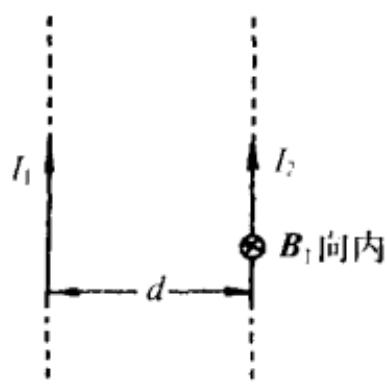
\includegraphics[width=0.5\linewidth]{figures/fig_6_2_31.jpg}
\end{center}

\vfill

\newpage

\textbf{6.2.32.} 发电厂的汇流条是两条三米长的平行铜棒,相距 50cm;当向外输电时,每条棒中的电流都是 10000A.作为近似,把两棒都当作无穷长的细导线,试估算它们之间相互作用力的大小.

\vfill

\textbf{6.2.33.} 两平行导线中电流方向相反时,它们便互相排斥.有一种磁悬浮列车便是利用这种排斥力使列车悬浮在车轨上运行的.设想两个相同的共轴圆线圈,半径都是R,匝数都是N,相距为r,载有相反的电流I,如图6.2.33所示.假定一个线圈中的电流在另一线圈中产生的磁感强度的大小可近似当作

$$
B = \frac {\mu_ {0} N I}{2 \pi r}
$$


试估算在 $r=10cm, R=1.0m$ 时，要使排斥力为 F=10 吨力，所需的安匝数 NI.

图6.2.33
\begin{center}
    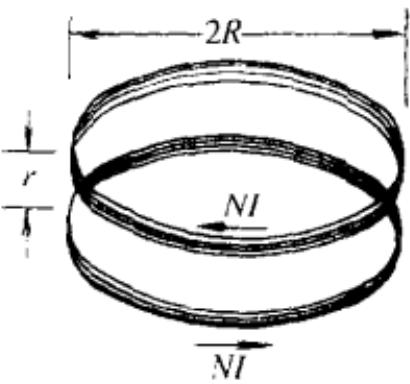
\includegraphics[width=0.5\linewidth]{figures/fig_6_2_33.jpg}
\end{center}

\vfill

\newpage

\textbf{6.2.34.} 两个平行的无穷长导体薄片, 宽度都是 $b$ , 相距为 $a$ , 分别载有方向相反的电流 $I_{1}$ 和 $I_{2}$ , 其横截面如图 6.2.34(1) 所示. 设 $I_{1}$ 和 $I_{2}$ 都均匀分布在各自的片上, 片的厚度均可略去不计. 试证明: 每片上单位长度受另一片的作用力的大小为

图6.2.34(1)

$$
F = \frac {2 \times 1 0 ^ {- 7} I _ {1} I _ {2}}{b ^ {2}} \left[ 2 b \arctan \left(\frac {b}{a}\right) - a \ln \left(\frac {a ^ {2} + b ^ {2}}{a ^ {2}}\right) \right]
$$

力的方向是互相排斥.

\vfill

\textbf{6.2.35.} 同轴电缆由长直圆柱导体和套在它外面的同轴导体薄圆筒构成, 已知圆筒的半径为 R, 其厚度可略去不计. 电流 I 沿轴线方向流动, 从圆柱流去, 沿圆筒流回, I 都均匀分布在横截面上. 试求圆筒单位面积上所受的力.

图6.2.35
\begin{center}
    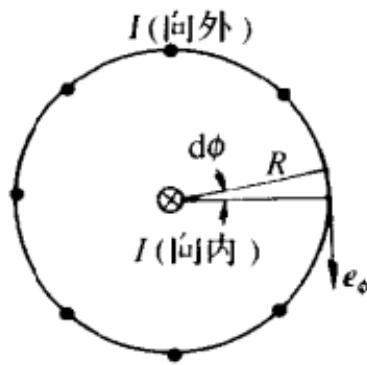
\includegraphics[width=0.5\linewidth]{figures/fig_6_2_35.jpg}
\end{center}

\vfill

\newpage

\textbf{6.2.36.} 如图 6.2.36, 一无限长直导线 $L_{1}$ 载有电流 $I_{1} = 2.0\mathrm{A}$ , 旁边有一段与它垂直且共面的一段导线 $L_{2}, L_{2}$ 长为 $l = 40\mathrm{cm}$ , 载有电流 $I_{2} = 3.0\mathrm{A}$ , 靠近 $L_{1}$ 的一端到 $L_{1}$ 的距离也是 $l = 40\mathrm{cm}$ . 试求 $L_{1}$ 上的电流作用在 $L_{2}$ 上的力.

\vfill

\textbf{6.2.37.} 设 $I_{1} \mathrm{d} l_{1}$ 和 $I_{2} \mathrm{d} l_{2}$ 分别为载流导线 $I_{1}$ 和 $I_{2}$ 上的任意两个电流元，从 $I_{1} \mathrm{d} l_{1}$ 到 $I_{2} \mathrm{d} l_{2}$ 的位矢为 $r_{12}$ ，如图6.2.37所示。试分别求 $I_{1} \mathrm{d} l_{1}$ 作用在 $I_{2} \mathrm{d} l_{2}$ 上的力和 $I_{2} \mathrm{d} l_{2}$ 作用在 $I_{1} \mathrm{d} l_{1}$ 上的力，并从而得出：它们之间的相互作用力一般不遵守牛顿第三定律。
\begin{center}
    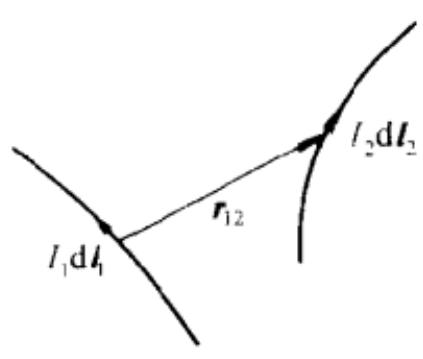
\includegraphics[width=0.5\linewidth]{figures/fig_6_2_37.jpg}
\end{center}

\vfill

\newpage

\textbf{6.2.38.} 任意两个闭合回路 $L_{1}$ 和 $L_{2}$ .

电流分别为 $I_{1}$ 和 $I_{2}$ , 如图6.2.38所示. 试证明: $L_{1}$ 作用在 $L_{2}$ 上的力 $\mathbf{F}_{21}$ 与 $L_{2}$ 作用在 $L_{1}$ 上的力 $\mathbf{F}_{12}$ 遵守牛顿第三定律, 即 $\mathbf{F}_{12} = -\mathbf{F}_{21}$ .

\vfill

\textbf{6.2.39.} 长直导线与一正方形线圈在同一平面内, 它们分别载有电流 $I_{1}$ 和 $I_{2}$ ; 正方形的边长为 $a$ , 有两边与导线平行, 它的中心 $O$ 到直导线的垂直距离为 $d$ , 如图 6.2.39 所示. (1) 试求这正方形载流线圈各边受 $I_{1}$ 的作用力以及这些力的主矢 (即这些力的矢量和); (2) 当 $I_{1} = 3.0 \mathrm{~A}, I_{2} = 2.0 \mathrm{~A}, a = d = 4.0 \mathrm{~cm}$ 时, 试计算主矢的大小.
\begin{center}
    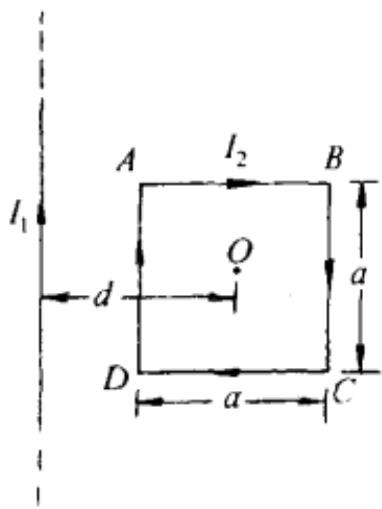
\includegraphics[width=0.5\linewidth]{figures/fig_6_2_39.jpg}
\end{center}

\vfill

\newpage

\textbf{6.2.40.} 一无穷长直导线载有电流 $I_{1}$ , 旁边有一正方形线圈ABCD载有电流 $I_{2}$ , 正方形边长为 $2a$ , 中心到直导线的垂直距离为 $b$ , 电流的方向如图6.2.40(1)所示. 线圈可以绕平行于直导线的轴 $P_{1}P_{2}$ 转动, $P_{1}P_{2}$ 通过线圈上下两边的中点.


试求:(1)线圈在 $\alpha$ 角度位置时[如图 6.2.40(1)所示], $I_{1}$ 作用在线圈各边上的安培力之和;(2)这些力对转轴 $P_{1}P_{2}$ 的力矩之和;(3)线圈平衡时 $\alpha$ 的值;(4)线圈从平衡位置转到 $\alpha=\frac{\pi}{2}$ 时, $I_{1}$ 作用在线圈上的力做了多少功?
\begin{center}
    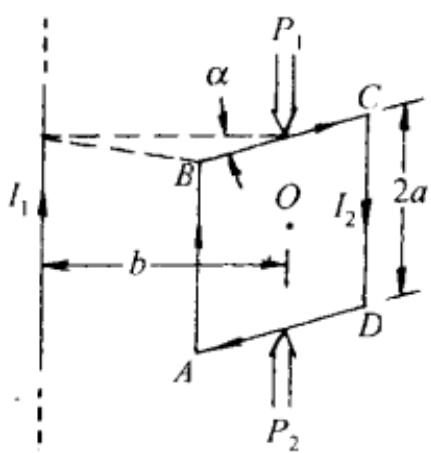
\includegraphics[width=0.5\linewidth]{figures/fig_6_2_40.jpg}
\end{center}

\vfill

\textbf{6.2.41.} 一无穷长直导线载有电流 $I_{1} = 30\mathrm{A}$ ，一长方形回路ABCD和它在同一平面内，且DA边与导线平行，线圈长为 $a = 30\mathrm{cm}$ ，宽为 $b = 8.0\mathrm{cm}$ ，一边到直导线的距离为 $c = 1.0\mathrm{cm}$ ，载有电流 $I_{2} = 20\mathrm{A}$ ，如图6.2.41所示。试求直导线上的电流作用在回路各边上的安培力之和。

\vfill

\newpage

\textbf{6.2.42.} 载有电流 $I_{1}$ 的无穷长直导线旁，有一与它共面的正三角形线圈，边长为 $a$ ，载有电流 $I_{2}$ ，一边与它平行，中心 $O$ 到它的距离为 $b$ ，如图6.2.42(1)所示.试求直导线上的电流 $I_{1}$ 作用在三角形线圈上各边的安培力之和.

\vfill

\textbf{6.2.43.} 一无穷长直导线载有电流 $I_{1}$ , 旁边有一个与它共面的圆线圈, 圆线圈的半径为 R，载有电流 $I_{2}$ ，圆心 O 到直导线的距离为 l，电流的方向如图 6.2.43(1) 所示。试求直线电流 $I_{1}$ 作用在圆线圈上的力。

图6.2.43(1)

图6.2.43(2)
\begin{center}
    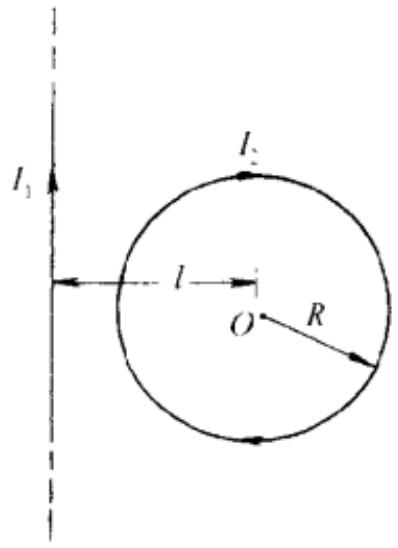
\includegraphics[width=0.5\linewidth]{figures/fig_6_2_43_1.jpg}
\end{center}
\begin{center}
    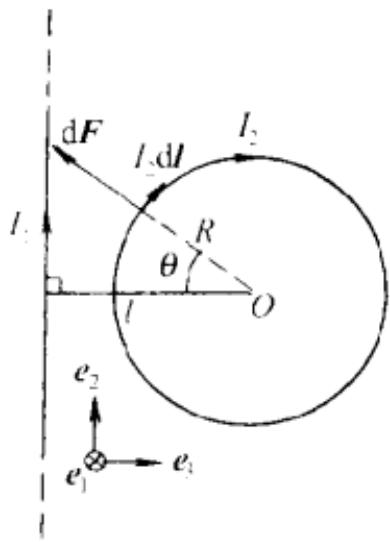
\includegraphics[width=0.5\linewidth]{figures/fig_6_2_43_2.jpg}
\end{center}

\vfill

\newpage

\textbf{6.2.44.} 两个圆线圈的半径分别为 $R_{1}$ 和 $R_{2}$ , 所载电流分别 $I_{1}$ 和 $I_{2}$ , 圆心相距为 $l$ , 线圈 2 的直径在线圈 1 的轴线上, 如图 6.2.44 所示. 当 $l$ 比 $R_{1}$ 和 $R_{2}$ 都大很多时, 试求 $I_{1}$ 作用在线圈 2 上的力矩.

图6.2.44
\begin{center}
    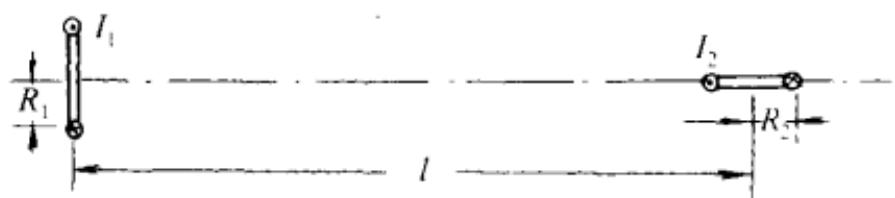
\includegraphics[width=0.5\linewidth]{figures/fig_6_2_44.jpg}
\end{center}

\vfill
